%%% Содержимое слайдов

\frame[plain]{\titlepage} % Титульный слайд

%-------------------------------------------------------------------------------

\section{Цели и задачи исследования}

\begin{frame}
\frametitle{\insertsection}

\textbf{Цель:} разработка системы для прогнозирования и обнаружения неисправностей
на станках лазерной резки Навигатор КС-12В компании ВНИТЭП

\vspace{\baselineskip}

\textbf{Задачи:}
\begin{itemize}
    \item анализ предметной области;
    \item обработка и подготовка накопленных данных со станка Навигатор КС-12В;
    \item выбор и обоснование выбора метода кластеризации;
    \item выбор и обоснование выбора модели предсказания;
    \item интеграция разработанного решения в систему компании Omnicube.
\end{itemize}
\end{frame}

%-------------------------------------------------------------------------------

\section{Станок лазерной резки Навигатор КС-12В}

\begin{frame}
\frametitle{\insertsection}

\begin{figure}
    \center
    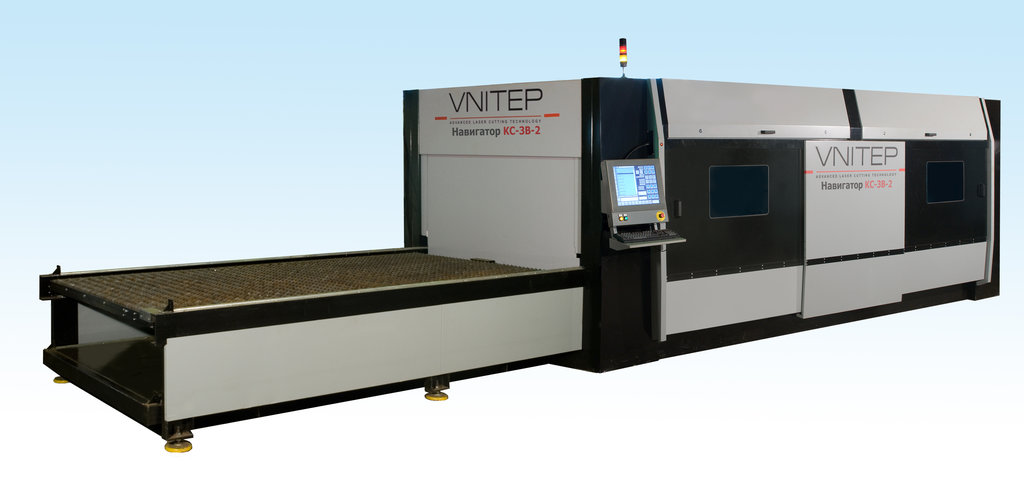
\includegraphics[width=10cm]{navigator.jpeg}
\end{figure}

\end{frame}

%-------------------------------------------------------------------------------

\section{Станок лазерной резки Навигатор КС-12В}

\begin{frame}
\frametitle{\insertsection}

\begin{figure}
    \center
    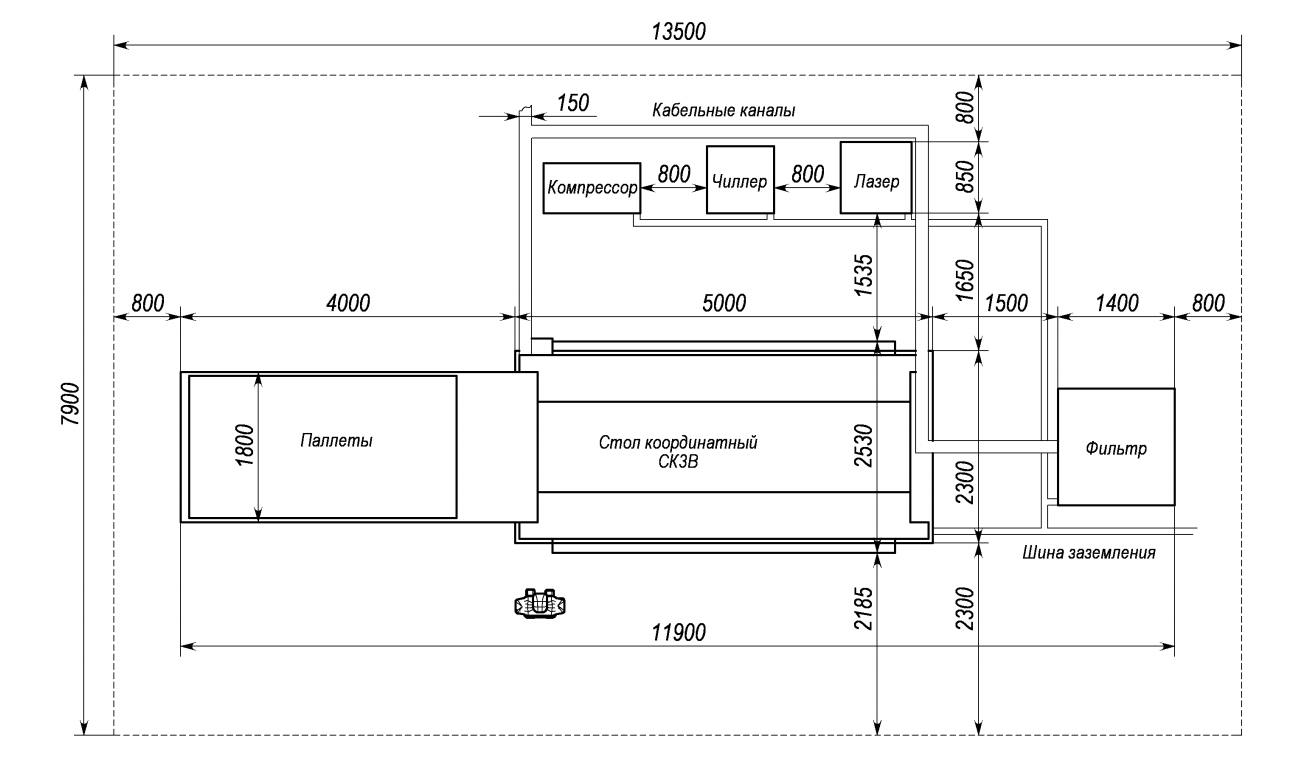
\includegraphics[width=10cm]{navigator.png}
\end{figure}
\end{frame}

%-------------------------------------------------------------------------------

\section{Система сбора данных Omnicube для компании Сеспель}

\begin{frame}
\frametitle{\insertsection}

\begin{figure}
    \center
    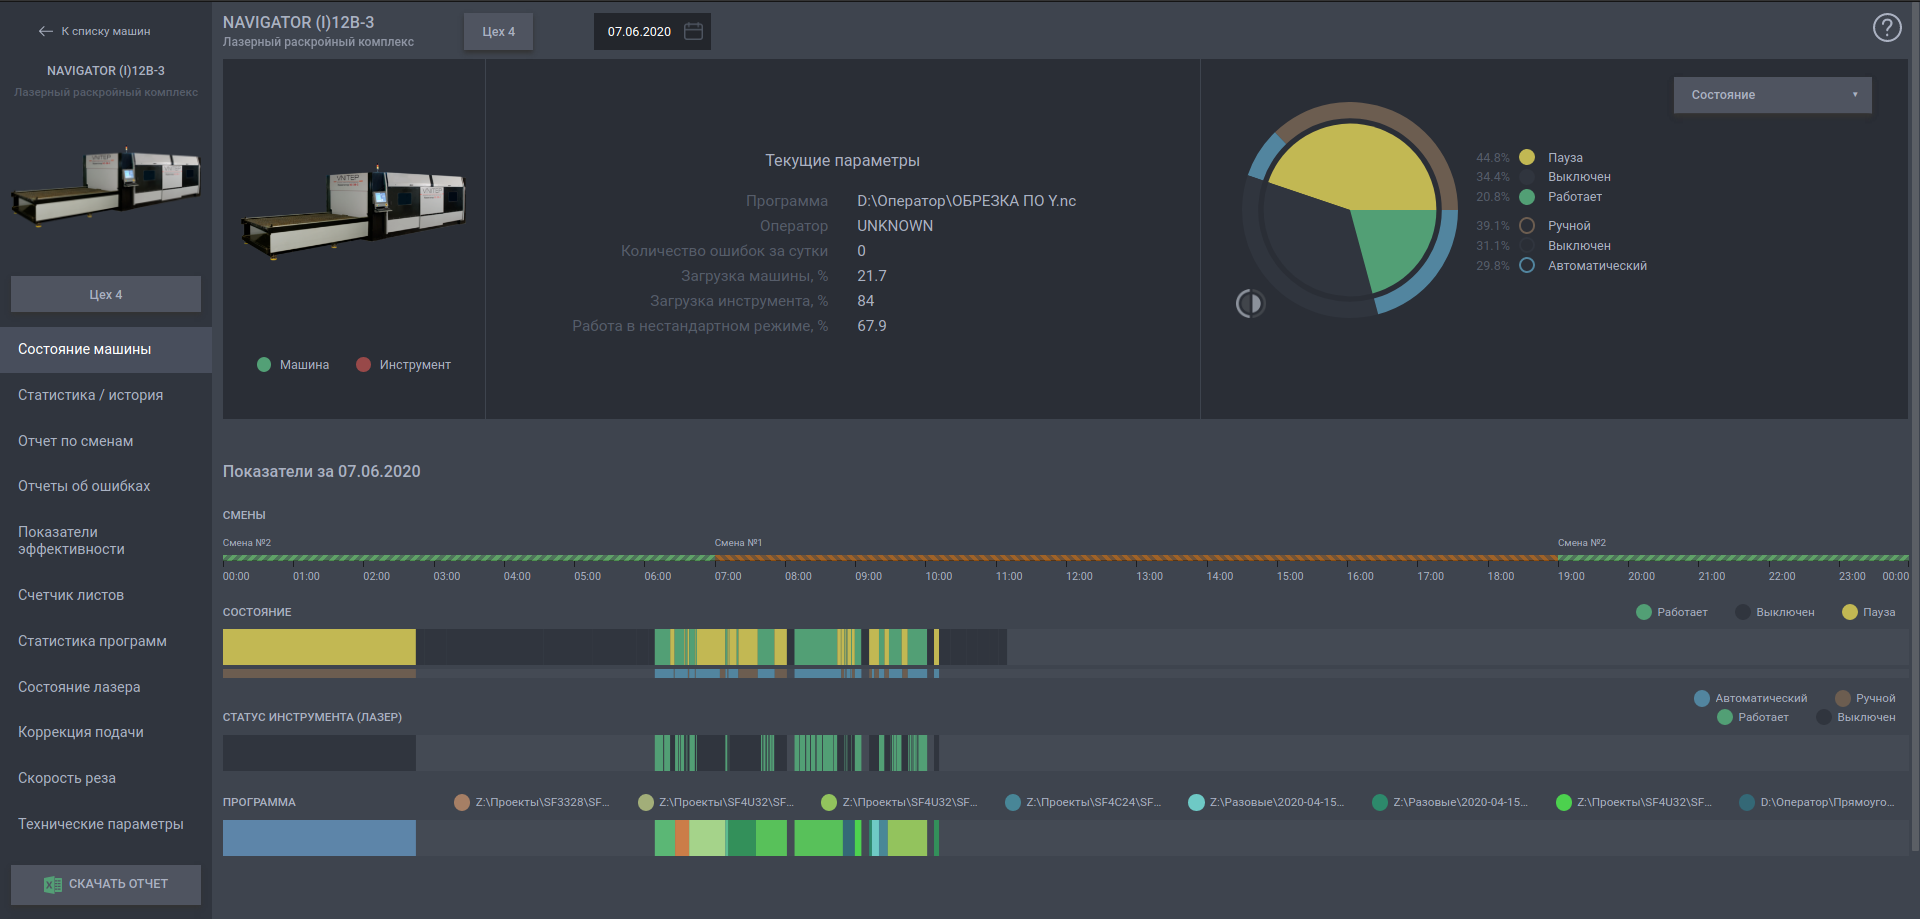
\includegraphics[width=11cm]{general.png}
\end{figure}

\begin{figure}
    \center
    
\includegraphics[width=2cm]{omnicube.png}
    \hfill
    
\includegraphics[width=2cm]{sespel.png}
\end{figure}

\end{frame}

%-------------------------------------------------------------------------------

\section{Проблема обнаружения неисправностей}

\begin{frame}
\frametitle{\insertsection}

\textbf{Недостатки существующих подходов:}
\begin{itemize}
    \item высокая стоимость диагностики и обнаружения неисправностей;
    \item необходимость наличия квалифицированного инженера на производстве;
    \item большое количество затрачиваемого времени;
    \item человеческий фактор.
\end{itemize}

\end{frame}

%-------------------------------------------------------------------------------

\section{Входные и выходные данные}

\begin{frame}
\frametitle{\insertsection}

\textbf{Входные данные:}
\begin{itemize}
    \item статус станка (режим работы);
    \item состояние лазера (мощность, температура);
    \item отчеты об ошибках во время работы станка;
    \item счетчик металлических листов.
\end{itemize}

\vspace{\baselineskip}

\textbf{Выходные данные:}
\begin{itemize}
    \item предсказанный отрезок данных;
    \item ПО для получения данных об уязвимостях
    \item анализ ПО используемого в облачных вычислениях
    \item информация о проблемах безопасности в облачной среде
\end{itemize}

\end{frame}

%-------------------------------------------------------------------------------
